\documentclass[]{article}
\usepackage[spanish.mexico]{babel}
\usepackage[T1]{fontenc}
\usepackage[utf8]{inputenc}
\usepackage{lmodern}
\usepackage[a4paper]{geometry}

%\usepackage{natbib}
\usepackage{cite}


%Grafico de barras
\usepackage{pgfplots}


\title{Proyecto de Optimización de Energía}
\author{Pablo Vivar Colina}
\date{Mayo 2018}

\begin{document}

\maketitle

\section{Introducción}

En física, energía se define como la capacidad para realizar un trabajo. En tecnología y economía, \textit{energía} se refiere a un recurso natural (incluyendo a su tecnología asociada) para poder extraerla, transformarla y darle un uso industrial o económico.\cite{EnergiaWiki}\\


\section{Objetivo}

En el siguiente proyecto el objetivo a lo largo del semestre era aplicar medidas para lograr el ahorro de energía, que como recurso natural es importante tener en cuenta que su generación implica un impacto medio ambiental, y si su consumo es reducido y o optimizado deberá verse reflejado.\\

\section{Consumo de energía Dispositivos}


\subsection{Lámpara Incandescente}

Una bombilla de incandescencia o bombilla incandescente es un dispositivo que produce luz mediante el calentamiento por efecto Joule de un filamento metálico, en concreto de wolframio, hasta ponerlo al rojo blanco, mediante el paso de corriente eléctrica. Con la tecnología existente, actualmente se considera poco eficiente, ya que el 85 $\%$ de la electricidad que consume la transforma en calor y solo el 15 $\%$ restante en luz.\cite{LamparaIncandescente}

\subsection{Lámpara fluorescente compacta}

La lámpara fluorescente compacta o lámpara fluocompacta (LFC) es un tipo de lámpara que aprovecha la tecnología de los tradicionales tubos fluorescentes para hacer lámparas de menor tamaño que puedan sustituir a las lámparas incandescentes con pocos cambios en la armadura de instalación y con menor consumo. La luminosidad emitida por un fluorescente depende de la superficie emisora, por lo que este tipo de lámparas aumentan su superficie doblando o enrollando el tubo de diferentes maneras. Otras mejoras en la tecnología fluorescente han permitido asimismo aumentar el rendimiento luminoso máximo desde los 40-50 lm/W hasta los alcanzar 80 lm/W, aunque su eficacia media actual en el mercado es de en torno a los 58 lm/W, que ha sido superado ampliamente por muchas lámparas tipo LED. También la sustitución de los antiguos electromagnéticos por balastros electrónicos ha permitido reducir el peso y el característico parpadeo de los fluorescentes tradicionales.\cite{LamparaFLuorescente}\\

En comparación con las lámparas incandescentes, las LFC tienen una vida útil más larga y consumen menos energía eléctrica para producir la misma cantidad de luz. Como desventajas, su reproducción de los colores, aunque actualmente es buena (IRC>80), no alcanza el espectro continuo de las incandescentes o halógenas (IRC=100), normalmente no alcanzan su máximo brillo de forma inmediata y es más problemático deshacerse de las viejas, pues hay que llevarlas a lugares específicos, ya que contienen residuos tóxicos. Además no es adecuado su uso en lugares cerrados pequeños o con temperatura alta, ya que se reduce drásticamente la duración por el rápido deterioro de la electrónica pudiendo llegar a explotar por sí solas bajo condiciones muy extremas.\cite{LamparaFLuorescente}\\


\subsection{Lámpara LED}

Una lámpara de ledes, también conocida como lámpara de tecnología led o más simplemente lámpara led (con led como la sigla de la tecnología de diodo emisor de luz, light emitting diode, en este caso idealmente en mayúsculas), es una lámpara de estado sólido que usa ledes (light-emitting diode, diodos emisores de luz) como fuente lumínica. Debido a que la luz capaz de emitir un led no es muy intensa, para alcanzar la intensidad luminosa similar a las otras lámparas existentes como las incandescentes o las fluorescentes compactas las lámparas led están compuestas por agrupaciones de ledes, en mayor o menor número, según la intensidad luminosa deseada.\cite{LamparaLED}

\section{Consumo hogar}

Podemos ver la distribución de las lámparas en el hogar con la figura \ref{fig:lámparas}, y además se puede apreciar un listado de los dispositivos que integran el funcionamiento el hogar en el cuadro \ref{tablaConsumo}.\\

La suma de las potencias los electrodomésticos usados en el hogar es de 2250 [W].\\


\begin{figure}
    \centering
    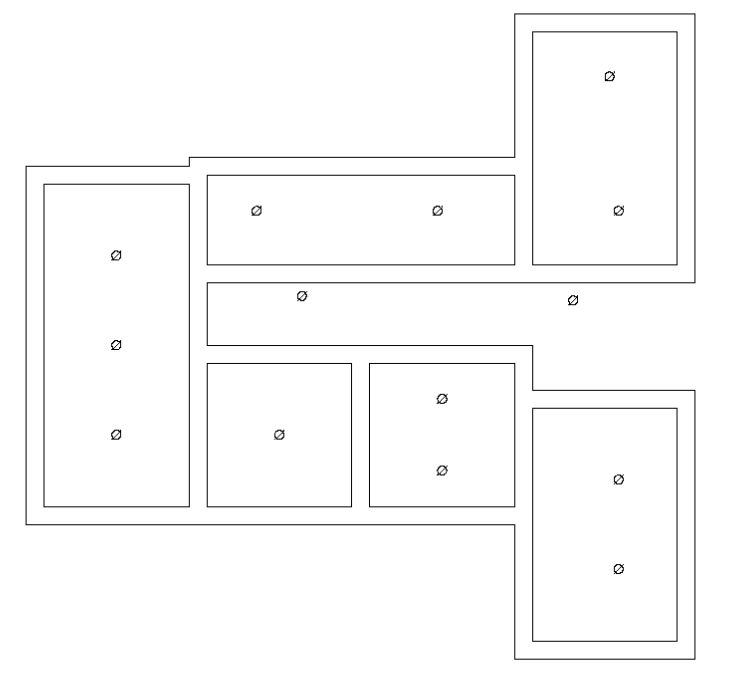
\includegraphics[width=0.3\textwidth]{Croquis}
    \caption{Esquema sencillos disposición de lámparas}
    \label{fig:lámparas}
\end{figure}

%Teniendo en cuenta la suma de potencias obtenidas



\begin{table}[h!]
\centering

\begin{tabular}{|c|c|c|c|c|}
\hline
Dispositivo           & Descripción                     & Cant. & Consumo {[}W{]} & Total [W] \\ \hline
Lámpara Incandescente & Bombilla filamento de tungsteno & 2                  & 75              & 150           \\ \hline
Lámpara ahorradora    & Bombilla fluorescente compacta  & 10                 & 18              & 180           \\ \hline
Lámpara led           & Bombilla luz led                & 5                  & 9               & 45            \\ \hline
Microondas            & Horno de microondas             & 1                  & 1200            & 1200          \\ \hline
Refrigerador          & Aparato Refrigerador            & 1                  & 540             & 540           \\ \hline
Computadoras          & Consumo de energía aparatos     & 3                  & 25              & 75            \\ \hline
Impresoras 3D         & Energía impresión 3D            & 2                  & 30              & 60            \\ \hline
\end{tabular}
\caption{Consumo en [W] del hogar al inicio del experimento}
\label{tablaConsumo}
\end{table}


%\begin{figure}[h!]
%	\centering
%	\begin{tabular}[]{|c|c|c|c|}
%		\hline
%		 Dispositivo & Descripción & Cantidad & Consumo \\
%		 	\hline
%		  \\
%		  \\
%		\hline
%	\end{tabular}
%	\label{cuadro:suministros}
%	\caption{Suministros}
	
%\end{figure}

\section{Suministro de Energía
}


\begin{figure}[h!]
	\centering
	\begin{tabular}[]{|c|c|}
		\hline
		 Suministro & Precio (MXN)\\
		 	\hline
		 Básico & 0.793 \\
		 Intermedio & 0.956 \\
		\hline
	\end{tabular}
	\label{cuadro:suministros}
	\caption{Suministros}
	
\end{figure}



\section{Historial de consumo de energía}

Según podemos ver en el cuadro \ref{cuadro:ultimosPeriodos} de los últimos periodos podemos ver que se miden cada dos meses, por lo que la energía mostrada en cada barra de la figura \ref{fig:grafConsumo} representa un periodo de 2 meses, en el cuadro \ref{cuadro:ultimosPeriodos} podemos apreciar los últimos 3 periodos de consumo de energía.\\



\begin{figure}[h!]
	\centering
\begin{tikzpicture}
\begin{axis}[
symbolic x coords={A,B,C,D,E,F,G,H,I,J,K},
xtick=data
]
\addplot[ybar,fill=orange] coordinates {
	(A,   291)
	(B,  284)
	(C,   323)
	(D,323)
	(E,339)
	(F,306)
	(G,254)
	(H,282)
	(I,302)
	(J,264)
	(K,272)
};
\end{axis}
\end{tikzpicture}
\caption{Consumo energía eléctrica [kWh]}
\label{fig:grafConsumo}
\end{figure}

\begin{figure}[h!]
	\centering
	\begin{tabular}[]{|c|c|c|}
		\hline
		Nombre & Periodo & Energía consumida [kWh]\\
		\hline
	I & 11/8/17-12/10/17 & 323 \\
	
	J & 12/10/17-11/10/17 & 284 \\
		K & 11/12/17-12/2/18 & 291 \\
	
		\hline
	\end{tabular}
	\label{cuadro:ultimosPeriodos}
	\caption{Últimos periodos}
	
\end{figure}

\section{Ahorro de energía}

De acuerdo con la sección del consumo del hogar podemos decir que se necesitan 17 bombillos, 2 de ellos incandescentes, 10 de ellos con bombilla fluorescente compacta y 5 de ellos de luz led.

Por lo que para un primer experimento de ahorro de energía se busca reducir la cantidad de bombillos de luz incandescente, y de luz fluorescente compacta para ser reemplazados por bombillos de luz LED preferentemente.\\

Se puede apreciar en un segundo cuadro \ref{tablaConsumoSegundo} que de los 17 focos que se necesitan en el hogar, los focos de luz incandescente han sido eliminados, y los bombillos de luz fluorescente compacta han sido reducidos, por último podemos apreciar que se aumentaron el uso de bombillos de luz LED.\\

La suma de las potencias de consumo del cuadro \ref{tablaConsumoSegundo} es de 2055 [W], comparada con la suma de potencias anteriores de 2250 [W], podemos notar una diferencia de 205 [W].\\

Se puede apreciar que del periodo I al periodo J existió un ahorro de 39 [kWh], y de el periodo J al K aumentó el consumo de energía 7 [kWh]. Pero si se revisa el historial anterior se puede apreciar que dentro de los bimestres anteriores el consumo de energía no había sido más bajo.\\

\begin{table}[h!]
\centering

\begin{tabular}{|c|c|c|c|c|}
\hline
Dispositivo           & Descripción                     & Cant. & Consumo {[}W{]} & Total [W] \\ \hline
Lámpara Incandescente & Bombilla filamento de tungsteno & 0                  & 75              & 0           \\ \hline
Lámpara ahorradora    & Bombilla fluorescente compacta  & 5                 & 18              & 90           \\ \hline
Lámpara led           & Bombilla luz led                & 10                  & 9               & 90            \\ \hline
Microondas            & Horno de microondas             & 1                  & 1200            & 1200          \\ \hline
Refrigerador          & Aparato Refrigerador            & 1                  & 540             & 540           \\ \hline
Computadoras          & Consumo de energía aparatos     & 3                  & 25              & 75            \\ \hline
Impresoras 3D         & Energía impresión 3D            & 2                  & 30              & 60            \\ \hline
\end{tabular}
\caption{Consumo en [W] del hogar al final del experimento}
\label{tablaConsumoSegundo}
\end{table}


\section{Conclusión}

Para éste experimento se realizo la medición del consumo de energía bajo estrictas restricciones.

\bibliographystyle{plain}
\bibliography{Referencias.bib}
%\addbibresource{Referencias.bib}

\end{document}
